\documentclass[11pt,letterpaper]{article}
\usepackage[T1]{fontenc}
\usepackage{lmodern}
\usepackage[margin=1in,headheight=15pt]{geometry}
\usepackage{amsmath,amssymb,bm,mathtools,microtype}
\usepackage{booktabs,tabularx,array,enumitem,needspace}
\usepackage{tikz,fancyhdr,xcolor,listings}
\usetikzlibrary{arrows.meta,calc}
\definecolor{linkblue}{RGB}{29,62,96}
\usepackage[colorlinks=true,linkcolor=linkblue,urlcolor=linkblue,citecolor=linkblue,menucolor=linkblue]{hyperref}
\usepackage[nameinlink,noabbrev]{cleveref}
\hypersetup{pdftitle={Fixed-Orientation Sliding Blocks: Contact Geometry, Guide Wrench and the CINDER Boundary},pdfauthor={CINDER technical note}}
\setlength{\parindent}{0pt}\setlength{\parskip}{.45em}
\setlength{\emergencystretch}{2em}
\clubpenalty=10000\widowpenalty=10000
\numberwithin{equation}{section}
\setlist{itemsep=.3em,topsep=.3em}
\pagestyle{fancy}\fancyhf{}
\fancyhead[L]{\small CINDER / Fixed-orientation sliding blocks}
\fancyhead[R]{\small CINDER 1.2.0}
\fancyfoot[L]{\small\Acrobatmenu{GoBack}{Previous view}}
\fancyfoot[C]{\thepage}\fancyfoot[R]{\small\hyperlink{contents}{Contents}}
\newcommand{\half}{\tfrac12}
\newcommand{\dd}{\mathrm d}
\newcommand{\er}{\bm e_r}\newcommand{\et}{\bm e_t}\newcommand{\ez}{\bm e_z}
\newcolumntype{Y}{>{\raggedright\arraybackslash}X}
\lstset{basicstyle=\small\ttfamily,breaklines=true,columns=fullflexible,frame=single}
\begin{document}
\begin{center}
{\small CINDER TECHNICAL NOTE / OCTOBER 11, 2026}\par\vspace{.7em}
{\LARGE\bfseries Fixed-Orientation Sliding Blocks}\par\vspace{.4em}
{\large Contact Geometry, Guide Wrench, and the Common Boundary}
\end{center}

A sliding centrifugal weight can move outward while two surfaces determine its
axial position. The fixed cup carries one surface; the movable sheave carries
the other. Once a guide prevents relative rotation of the weight, those two
contact constraints can determine its translation from sheave closure alone.
The resulting motion supplies the same effective mass and shaft inertia as
any other mechanism admitted by the common boundary \cite{common}.

That reduction does not make the block torque-free. Contact forces generally
have different moment arms about its centre of mass (COM), and the block still
rotates in space with the shaft. This note derives the contact motion first,
then the inertia functions, complete ideal-guide demand, and the impulses
needed to retain the contacts at a velocity reset.

The supported model is a CVTech-style sliding-block arrangement. The examples
are synthetic profiles, not measured CVTech hardware. A particular cup, weight,
insert, moving sheave, and anti-rocking guide still require their actual
geometry and mass properties before this model can represent that assembly.

\hypertarget{contents}{}\setcounter{tocdepth}{1}\tableofcontents
\clearpage
\section{Attachments, coordinates, and retained motion}

Use the right-handed local basis $(\er,\et,\ez)$, with $\ez$ along the shaft
and $\et=\ez\times\er$. The local sheave coordinate $x$ is positive in closure;
the moving contact track translates by $+x\ez$. The lower track is axially
fixed in the shaft frame. Both tracks and the orientation guide co-rotate
with the shaft at angular speed $\omega$ and acceleration $\alpha$.

Let $(R(x),Z(x))$ locate a datum fixed in the block. The block does not rotate
relative to these local axes. Its COM offset from the datum is the fixed
vector $(c_r,c_t,c_z)$, so the COM coordinates are
\begin{equation}
 r=R+c_r,\qquad y=c_t,\qquad z=Z+c_z.
\end{equation}
Separating this datum from the COM is essential for tuning inserts: changing
an insert can move the COM without moving either contacting face.

The complete identical set has mass $M$ and contains $n$ blocks. One block has
mass $M/n$. Store the centroidal inertia tensor per unit mass as $\bm K$,
expressed in $(r,t,z)$ axes. Thus $\bm I_{C,\mathrm{set}}=M\bm K$ is the sum of
corresponding local centroidal tensors, and $\bm I_{C,1}=M\bm K/n$ belongs to
one block. Off-diagonal entries are the entries of the inertia tensor itself:
for example, $K_{rz}=-\int u_r u_z\,\dd m/m$. They are not unsigned geometric
products of inertia.

The mass set is constant. The cup and rigid sheave masses remain in the host
pulley accounting; they are not included in $M$. Springs and belt loads are
separate elements. The contacts here are frictionless and unilateral. The
initial guide is an explicit ideal constraint: it supplies a tangential force
through the COM and an arbitrary holding couple, with no frictional loss.
Physical guide capacities are unknown, rather than inferred from the outline.

\section{Two finite profiles determine the body translation}
\label{sec:contacts}

Each contact face is a finite graph in a meridional section. Write the lower
and upper block faces as $z=b_\ell(u)$ and $z=b_u(u)$, where $u$ is radial
position relative to the body datum. The two faces share a declared interval
$[u_a,u_b]$, and $b_u>b_\ell$ throughout it. The fixed and moving tracks are
$z=f_\ell(\rho)$ and $z=f_u(\rho)+x$, respectively, on finite radial domains.
The whole block footprint must remain within both modelled track domains.

At a trial datum pose $(R,Z)$, define the signed axial gaps
\begin{align}
 g_\ell(u;R,Z)&=Z+b_\ell(u)-f_\ell(R+u),\\
 g_u(u;R,Z,x)&=f_u(R+u)+x-Z-b_u(u).
\end{align}
A nonnegative gap means separation without penetration. A retained contact
requires the minimum gap on that face to be zero. This compares the full
finite face, rather than selecting a tangent while ignoring another part of
the same face that might penetrate the track.

The implementation supports lines, quadratics, and circular-arc graphs:
\begin{align}
 f(\rho)&=f_0+s(\rho-\rho_0) &&\text{(line)},\\
 f(\rho)&=f_0+s(\rho-\rho_0)+\half k(\rho-\rho_0)^2
                &&\text{(quadratic)},\\
 f(\rho)&=f_0+\sigma\bigl[a-\sqrt{a^2-(\rho-\rho_0)^2}\bigr]
                &&\text{(circular arc)},
\end{align}
with $a>0$, $\sigma=\pm1$, and the circle's domain strictly inside
$|\rho-\rho_0|<a$. These are radial-coordinate graphs, not arbitrary rotated
arcs or a general CAD representation. Overhangs and saddle contacts require a
different contact construction.

\subsection{Selecting a branch without hiding another minimum}

The radial window $[R_{\min},R_{\max}]$ is part of the input. Exact bounds on
profile second derivatives determine whether each gap is convex or concave
over this window. A convex gap has its minimum at an endpoint or at its unique
stationary point; a concave gap has its minimum at an endpoint. An ambiguous
curvature bound is rejected. Strict derivative or endpoint-gap inequalities
then establish that the same endpoint or interior contact remains active
throughout the window. Conformal contacts and mode switches are rejected;
their pressure distribution or new branch cannot be obtained by blending the
old motion curves.

To reduce the two equations, put
\begin{equation}
 A(R)=\max_u[f_\ell(R+u)-b_\ell(u)],\qquad
 C(R)=\min_u[f_u(R+u)-b_u(u)].
\end{equation}
The lower contact gives $Z=A(R)$ and the upper contact gives
\begin{equation}
 x=A(R)-C(R).
 \label{eq:inverse}
\end{equation}
Disjoint track-slope bounds establish a nonzero derivative of this function
throughout the selected window. A bracketed scalar solve then gives the unique
$R$ in that window. This is a statement about the declared branch window, not
about every possible assembly elsewhere in the geometry.

Endpoint contact is allowed only when explicitly requested. It is an ideal
point contact at a finite face endpoint with the smooth track's normal.
A rounded nose of finite radius must be represented by its actual geometry
if its change to the contact path matters. Neither an unknown corner radius
nor a pressure centroid is fitted automatically.

\section{Motion ratios from the same contact constraints}

Let $u_\ell$ and $u_u$ be the active face coordinates and let
$s_i=f_i'(R+u_i)$ be the corresponding track slopes. At an interior tangent,
$b_i'(u_i)=f_i'(R+u_i)$. The derivative of the minimum gap with respect to its
minimizer vanishes; at a retained endpoint, $u_i$ is constant. In either case,
differentiating the two closed gaps gives
\begin{equation}
 Z'=s_\ell R',\qquad Z'=1+s_u R'.
\end{equation}
Consequently,
\begin{equation}
 D=s_\ell-s_u,\qquad R'=\frac1D,\qquad Z'=\frac{s_\ell}{D}.
 \label{eq:first}
\end{equation}
The constraint Jacobian has rows $(-s_\ell,1)$ and $(s_u,-1)$.
As $D$ approaches zero the geometry ceases to determine a regular translation.
The implementation bounds its condition number over the branch and rejects
ill-conditioned windows rather than clipping the motion ratio.

Curvature changes the active track slope as the block moves. At an interior
contact, differentiation of the tangency condition with respect to $R$ yields
\begin{equation}
 u_{i,R}=\frac{f_i''}{b_i''-f_i''},\qquad
 s_{i,R}=f_i''(1+u_{i,R}).
 \label{eq:contact-migration}
\end{equation}
At a retained endpoint $u_{i,R}=0$. All profile derivatives in this expression
are evaluated at the active material coordinates. Thus the second motion
ratios are
\begin{equation}
 R''=-(s_{\ell,R}-s_{u,R})(R')^3,\qquad
 Z''=s_\ell R''+s_{\ell,R}(R')^2.
 \label{eq:second}
\end{equation}
The fixed COM offset does not affect these derivatives: $r'=R'$, $z'=Z'$,
and likewise for second derivatives.

\section{Mass motion supplies the four quantities}
\label{sec:inertia}

Because orientation is fixed relative to the shaft frame, every material point
has the same relative translation velocity $(r',0,z')\dot x$. Its spin about
the COM still contributes to shaft-rotation energy. Integrating the material
velocity therefore gives
\begin{equation}
 T_f=\half M\bigl[(r')^2+(z')^2\bigr]\dot x^2
       -M c_t r'\omega\dot x
       +\half\bigl[M(r^2+c_t^2)+M K_{zz}\bigr]\omega^2.
\end{equation}
The mixed coefficient is $B_f=-M c_t r'$. Fixed orientation alone does not
remove it. The initial implementation requires $c_t=0$; it does not infer
cancellation from equally spaced blocks. With that condition established,
\begin{equation}
\boxed{\begin{aligned}
 M_f&=M[(r')^2+(z')^2],&
 M_f'&=2M(r'r''+z'z''),\\
 J_f&=Mr^2+M K_{zz},& J_f'&=2Mrr'.
\end{aligned}}
\label{eq:maps}
\end{equation}
These are total-set quantities. The count $n$ does not multiply them again.
The tensor must be finite and symmetric, with nonnegative principal inertias
satisfying the triangle inequalities. These checks establish a possible
inertia tensor; they do not establish that supplied mass properties actually
belong to the specified outline and inserts.

The common CINDER element \cite{common} consumes \cref{eq:maps} and supplies
\begin{equation}
 F_x=\half J_f'\omega^2-M_f\ddot x-\half M_f'\dot x^2,
 \qquad \tau=-J_f\alpha-J_f'\dot x\omega.
 \label{eq:loads}
\end{equation}
There is one implementation of these relations in
\texttt{CentrifugalInertiaForce}. The sliding-block provider adds the geometry
and contact policy; it does not carry another transient force law. The same
$M_f$ and $J_f$ enter kinetic energy and event projection.

\section{Contact reactions and the torque on each block}
\label{sec:wrench}

The four maps describe work and kinetic energy, but their reduction has
eliminated the individual constraint reactions. Recover those reactions from
the block's free body before deciding whether the contact branch is admissible.
The contact normals on the block, written as radial--axial pairs, are
\begin{equation}
 \bm n_\ell=\frac{(-s_\ell,1)}{\sqrt{1+s_\ell^2}},\qquad
 \bm n_u=\frac{(s_u,-1)}{\sqrt{1+s_u^2}}.
\end{equation}
With compression positive, the total corresponding normals satisfy
\begin{equation}
 [\bm n_\ell\ \bm n_u]
 \begin{bmatrix}N_\ell\\N_u\end{bmatrix}
 =M\begin{bmatrix}
 r'\ddot x+r''\dot x^2-r\omega^2\\
 z'\ddot x+z''\dot x^2
 \end{bmatrix}.
 \label{eq:normals}
\end{equation}
The tangential acceleration is separate. The ideal guide supplies
\begin{equation}
 G_t=M(r\alpha+2\omega r'\dot x).
 \label{eq:guide-force}
\end{equation}
The $2\omega r'\dot x$ term is the tangential acceleration associated with
radial motion in the rotating frame. Neither contact normal in this model has
a tangential component.

The guide must also prevent relative rocking. Let $\bm a_i$ run from the COM
to contact $i$, let $\bm N_i=N_i(n_{i,r},0,n_{i,z})$, and use the full
centroidal tensor. The required holding couple is
\begin{equation}
 \boxed{\bm G_C=M\bm K\,(\alpha\ez)
       +(\omega\ez)\times[M\bm K(\omega\ez)]
       -\sum_{i=\ell,u}\bm a_i\times\bm N_i.}
 \label{eq:guide-moment}
\end{equation}
The spin terms have components
\begin{equation}
 M\bigl(K_{rz}\alpha-K_{tz}\omega^2,\quad
        K_{tz}\alpha+K_{rz}\omega^2,\quad K_{zz}\alpha\bigr).
\end{equation}
Even at constant shaft speed, a nonzero product of inertia can require a
transverse couple. Even with zero products, the two contact moments need not
cancel. A single shaft-axis gyration radius cannot determine this full demand.

For the straight synthetic case at $x=7.5\,\mathrm{mm}$,
$r=57\,\mathrm{mm}$, $M=0.75\,\mathrm{kg}$ and
$\omega=350\,\mathrm{rad\,s^{-1}}$, steady contact gives
$F_x=2094.75\,\mathrm N$. The contact-only holding couple has magnitude
$51.0595\,\mathrm{N\,m}$ in corresponding local axes, or
$17.0198\,\mathrm{N\,m}$ per block for $n=3$.
\Cref{fig:fbd} shows why the lines of action do not remove this moment.

\begin{figure}[htbp]\centering
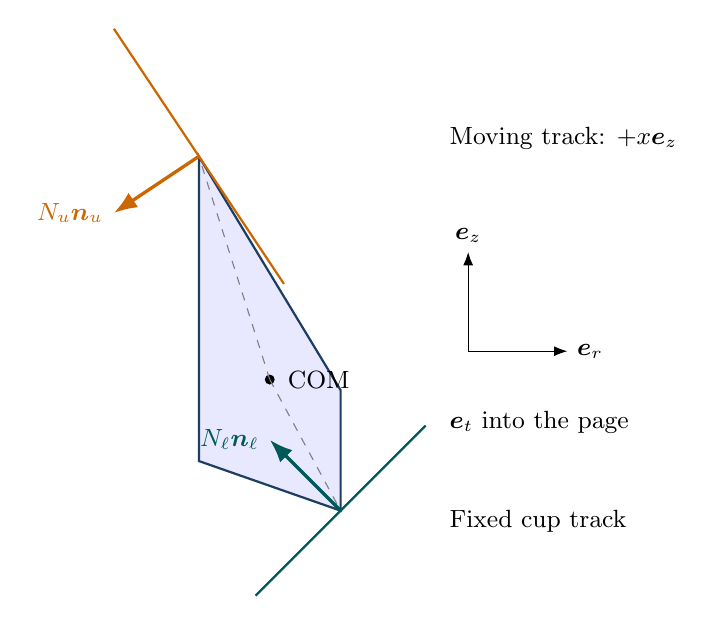
\begin{tikzpicture}[x=.18cm,y=.18cm,>=Latex,font=\small]
 \filldraw[fill=blue!9,draw=linkblue,thick] (-5,-5.75)--(5,-9.25)--(5,-.75)--(-5,15.75)--cycle;
 \draw[teal!70!black,thick] (-1,-15.25)--(11,-3.25);
 \draw[orange!80!black,thick] (-11,24.75)--(1,6.75);
 \fill (0,0) circle (.35) node[right=3pt]{COM};
 \draw[gray,dashed] (0,0)--(5,-9.25);
 \draw[gray,dashed] (0,0)--(-5,15.75);
 \draw[->,teal!70!black,very thick] (5,-9.25)--(0,-4.25) node[left]{$N_\ell\bm n_\ell$};
 \draw[->,orange!80!black,very thick] (-5,15.75)--(-11,11.75) node[left]{$N_u\bm n_u$};
 \node[anchor=west] at (12,17){Moving track: $+x\ez$};
 \node[anchor=west] at (12,-10){Fixed cup track};
 \draw[->] (14,2)--(21,2) node[right]{$\er$};
 \draw[->] (14,2)--(14,9) node[above]{$\ez$};
 \node[anchor=west] at (12,-3){$\et$ into the page};
\end{tikzpicture}
\caption{Local section of the straight synthetic block at the stated pose.
The contact arms are measured from the COM. Shaft-induced centripetal
acceleration is supplied by the resultant radial force; the guide couple must
balance the contact moment as well as any centroidal spin demand. The track
segments indicate contact surfaces, not complete cup or sheave solids.}
\label{fig:fbd}
\end{figure}

All normals and guide components above are sums of corresponding local values;
divide by $n$ for one pocket. They are not a global transverse-vector sum around
the pulley. Symmetric cancellation at assembly level does not unload each
pocket. Circumferential sidewall forces alone also cannot resist a moment
about the tangential axis: an anti-rocking feature must constrain that motion.
A specified real guide may transmit radial and axial forces too, in which case
\cref{eq:normals} must be replaced by the complete guide/contact equilibrium.

For the present ideal guide, the moving track delivers
$F_x=-N_u n_{u,z}$. This agrees with \cref{eq:loads} for the exact constraint
motion. The runtime contact policy uses both $N_\ell$ and $N_u$ at the actual
solved accelerations. It rejects tension; it never replaces a negative normal
by zero while retaining the same constrained mass map.

\section{Retaining the contacts through a velocity reset}
\label{sec:impact}

An instantaneous reset changes velocities at one fixed configuration. Smooth
centrifugal, Coriolis, spring, and applied-torque terms do not supply finite
impulses over that zero-duration interval. If the same two contacts and guide
remain active, their required impulses follow from the velocity jumps:
\begin{align}
 [\bm n_\ell\ \bm n_u]
 \begin{bmatrix}P_\ell\\P_u\end{bmatrix}
   &=M\begin{bmatrix}r'\\z'\end{bmatrix}\Delta\dot x,\\
 P_t&=Mr\Delta\omega,\\
 \bm L_C&=M\bm K(\Delta\omega\ez)
             -\sum_i\bm a_i\times\bm P_i.
 \label{eq:impulse}
\end{align}
The normal impulses must be compressive. The ideal guide is permitted to carry
its computed force impulse and couple impulse, but its real capacity is still
unknown. A positive running normal force does not establish the sign of these
impulses.

For the straight case, arresting $\dot x=+0.1\,\mathrm{m\,s^{-1}}$ with no
shaft-speed jump requires
\begin{equation}
 (P_\ell,P_u)=(-0.00848528,\ 0.04326662)\,\mathrm{N\,s}.
\end{equation}
The lower contact would have to pull. The stop therefore cannot retain this
branch, despite admissible pre-impact running forces. CINDER exposes the
normal-impulse margins on candidate projections and rejects an inadmissible
selected transition. Resolving what happens after release needs a different
contact topology or an additional dynamic coordinate; this version does not
invent that motion.

\section{Compilation, inputs, and limits in CINDER 1.2.0}

\texttt{SlidingBlockGeometry} stores the four profiles, radial branch window,
local axial interval, and explicit endpoint-contact policy.
\texttt{SlidingBlockMass} stores total mass, count, COM offset, and the full
centroidal tensor per mass. \texttt{SlidingBlockSpec} combines these with the
required \texttt{ideal\_fixed\_orientation} guide declaration.
The saved component kind is \texttt{sliding\_block\_flyweight}. Distances are
metres, mass is kilograms, profile curvature is inverse metres, and tensor
entries are square metres. The three JSON examples adjacent to the package
examples provide complete component records; they are not full CVT assemblies.

The compiler solves geometry outside the runtime RHS and constructs a common
$C^2$ piecewise quintic Hermite representation of $R,Z,u_\ell,u_u$. Values and
first two derivatives come from the same contact construction. Both inertia
functions and their derivatives use this one compiled motion. Contact
locations and normals also use the cached representation; no root solve is
performed inside the closure iteration.

Starting from eight intervals, the compiler tests three interior points per
cell and subdivides failed cells. Its absolute tolerances are
$2\times10^{-10}\,\mathrm m$ for positions,
$2\times10^{-7}$ for first derivatives, and
$2\times10^{-4}\,\mathrm{m^{-1}}$ for second derivatives.
The compilation report records the largest observed errors. These are sampled
interpolation diagnostics, distinct from the interval tests establishing the
contact branch; they are not rigorous continuum bounds on interpolation error.
The cache is keyed by the immutable geometry, so mass changes reuse the motion.
Queries outside the compiled axial interval raise an error without extrapolation.

\begin{center}\begin{tabularx}{\textwidth}{@{}p{.25\textwidth}Y@{}}
\toprule
Limit & Implemented response\\\midrule
Invalid inputs & Reject non-finite values, impossible tensors, nonpositive thickness,
invalid domains/count, and a nonzero tangential COM offset.\\[.4em]
Geometric branch & Reject unsupported gap curvature, ambiguous/conformal contact,
mode changes, insufficient track support, and ill-conditioned kinematics.\\[.4em]
Operating state & Evaluate both normal forces with the solved local acceleration;
reject contact loss. Report the complete ideal-guide demand separately.\\[.4em]
Velocity reset & Resolve both normal impulses and reject a selected reset requiring
tension. Direct projection callers must check the returned margins.\\[.4em]
Hardware envelope & Speed, stress, pressure, real guide capacity, supporting-solid
clearance, and three-dimensional interference require additional supplied data
and checks; no universal safe RPM is derived from these profiles.\\\bottomrule
\end{tabularx}\end{center}

The mechanism may mount on either pulley when both contact tracks co-rotate
with its shaft. A relative sheave helix is rejected. The host retains the full
local-to-shared acceleration relation and the separate sheave/cup mass
ownership. The frontend editor and authoritative preview service are a
subsequent application change. The research viewer now imports CINDER's Python
mechanics and contracts exported response coefficients in JavaScript; it does
not maintain another contact-force equation.

\section{Verification and what it establishes}

The straight case recovers the force form used in Messick's straight-ramp
model \cite{messick}: $M_f'=0$ and the steady closing force is $Mr r'\omega^2$,
with total $M$ replacing a per-weight mass times count. This tests the force
scale and geometry convention, not the dimensions of a particular machine.

The core smoke tests also differentiate inertial Cartesian trajectories of
eight material masses. Only direct geometric positions are reused; the
expected force, shaft torque and kinetic energy do not use the four-map
formula. Three profile families, forward/reverse/zero shaft rotation, and both
host shaft channels are exercised. Other checks cover derivative consistency,
COM changes at fixed geometry, opposite products of inertia at identical four
maps, saved-document/schema round trips, named running contacts, and valid and
invalid stop projections. A short coupled neutral-shift transient checks
primary angular-momentum conservation while axial motion changes shaft inertia.

The existing fixed-pivot launch regression remains a separate check of the
common-boundary migration. None of these checks measures real CVTech guide
capacity, contact pressure, wear, or post-release motion. Their practical
conclusion is that the stated constrained model supplies consistent continuous
and impulsive mechanics and explicitly identifies conditions it cannot retain.

\appendix
\section{Contact-coordinate derivatives for the interpolant}

The compiler also needs derivatives of the material contact coordinate. With
$h=u_R=f''/(b''-f'')$ at an interior tangent, another differentiation gives
\begin{equation}
 u_{RR}=\frac{f'''(1+h)^2-b'''h^2}{b''-f''},\qquad
 u'=hR',\qquad u''=hR''+u_{RR}(R')^2.
\end{equation}
All of these derivatives are zero for a retained material endpoint. Lines and
quadratics have zero third derivative. For the circle used in
\cref{sec:contacts}, with $d=\rho-\rho_0$,
\begin{equation}
 f''=\frac{\sigma a^2}{(a^2-d^2)^{3/2}},\qquad
 f'''=\frac{3\sigma a^2d}{(a^2-d^2)^{5/2}}.
\end{equation}
The open-semicircle domain and branch checks keep these values finite. A
contact-mode change requires a separate branch; this derivative construction
does not assign a smoothed corner motion.

\begin{thebibliography}{9}
\bibitem{common} \emph{General Centrifugal Mechanisms: From Compatible Motion to
Clamping Force and Shaft Coupling}. Revision 4; canonical CINDER 1.2.0 edition.
\href{../common_boundary/formulation.pdf}{Common-boundary document}.
\bibitem{fixed} \emph{Clamping Mechanism Implementations: The Fixed-Pivot Roller
Flyweight}. CINDER 1.2.0 edition.
\href{../fixed_pivot/formulation.pdf}{Fixed-pivot document}.
\bibitem{manuscript} Kai Arseneau and W. Spencer Smith.
\emph{A First-Principles Dynamic Model of a Rubber V-Belt CVT for General
Transient Simulation: With Mechanical Actuation and Traction-Limited Torque
Transfer}. Supplied manuscript, October 1, 2026; Sections 3.2, 3.3 and 3.6.
\bibitem{messick} M. J. Messick. Supplied 2018 thesis, Section 9.4.1,
printed page 109 (PDF page 118), Eq. 9.2. Used for the straight-ramp force limit;
the dimensions in this note are synthetic.
\end{thebibliography}
\end{document}
